\section{水能的利用}\label{sec:8-8}

唐诗中有“黄河远上白云间” 、“不尽长江滚滚来”的诗句。
这动人的诗句不但歌颂了孕育中华民族灿烂文化的黄河、长江的雄伟气势,
也生动形象地反映出这两条大河蕴藏着大量的势能和动能。
我们伟大的祖国,较大的河流有一千五百多条,水能蕴藏量达 6.8 亿千瓦,
其中可以开发利用的有 3.7 亿千瓦,居世界第一位。
为了节约煤炭、石油,应该优先开发水能资源,尽量利用水能做功。

利用水能做功,需要使用水力发动机。
早在 1900 多年以前,我们祖先就发明了简单的水力发动机,
用来汲水、磨粉、舂米、碾谷。图 \ref{fig:8-13} 所示的水磨就是一个例子。

\begin{figure}[htbp]
    \centering
    \begin{minipage}{7cm}
    \centering
    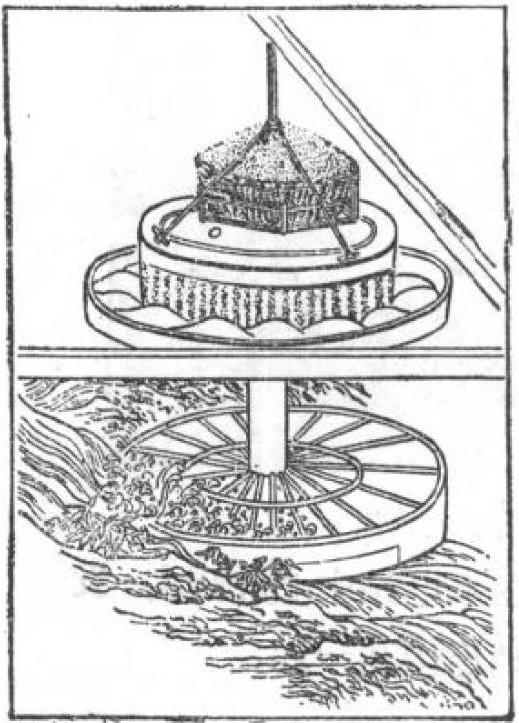
\includegraphics[width=5cm]{../pic/czwl1-ch8-13}
    \caption{水磨(采自古书《天工开物》)}\label{fig:8-13}
    \end{minipage}
    \qquad
    \begin{minipage}{7cm}
    \centering
    \vspace{6em}
    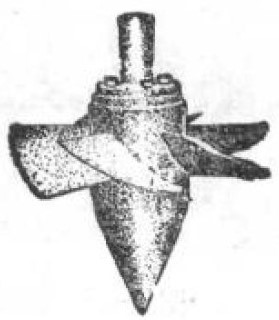
\includegraphics[width=4cm]{../pic/czwl1-ch8-14}
    \caption{轴流式水轮机的叶轮}\label{fig:8-14}
    \end{minipage}
\end{figure}


简单的水力发动机的机械效率很低,现代的水力发动机——水轮机的机械效率很高,可达 $90\%$ 以上。
图 \ref{fig:8-14} 是一种常见的轴流式水轮机的叶轮。它的轴竖直地装在轴承上,轴的下端有 3 ~ 6 片轮叶。
当水沿着轴的方向流来冲击轮叶的时候,水流的大部分动能传递给水轮机。
水轮机便转动起来,带动发电机发电。

水的动能越多,水轮机能够做的功就越多。
可是一般河流的河床比较平缓,流速不大,水的动能不多,
为了增加水的动能需要修筑拦河坝来提高上游的水位(图 \ref{fig:8-15})。
上游水位提得越高,上游水的势能就越多,水从上游流下来的时候,由势能转化成的动能也越多,
有的大型水电站的拦河坝修得很高,甚至超过三百米。

\begin{figure}[htbp]
    \centering
    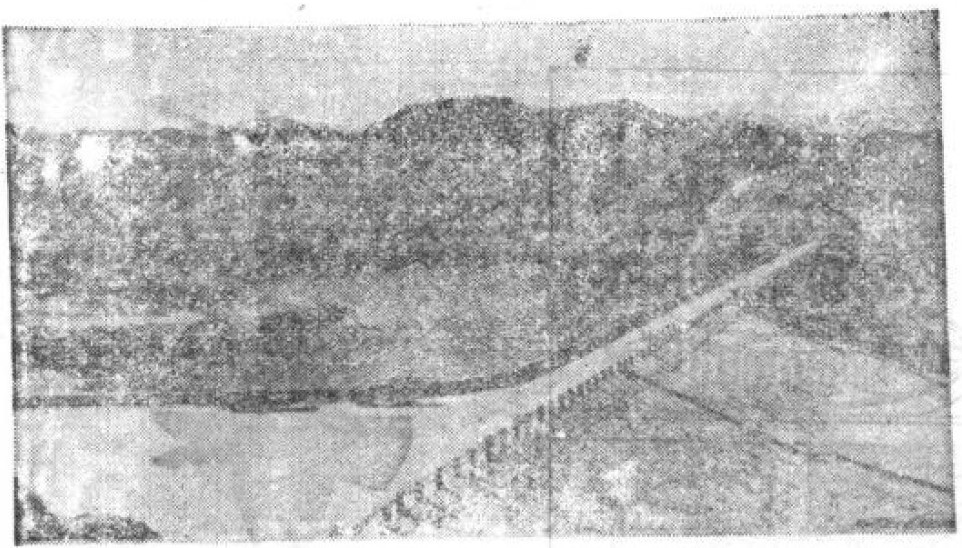
\includegraphics[width=0.8\textwidth]{../pic/czwl1-ch8-15}
    \caption{刘家峡水电站的拦河坝}\label{fig:8-15}
\end{figure}


图 \ref{fig:8-16} 表示水轮机安装在水电站中的情形。
发电机装在水轮机上面,它们的轴连接在一起。

\begin{figure}[htbp]
    \centering
    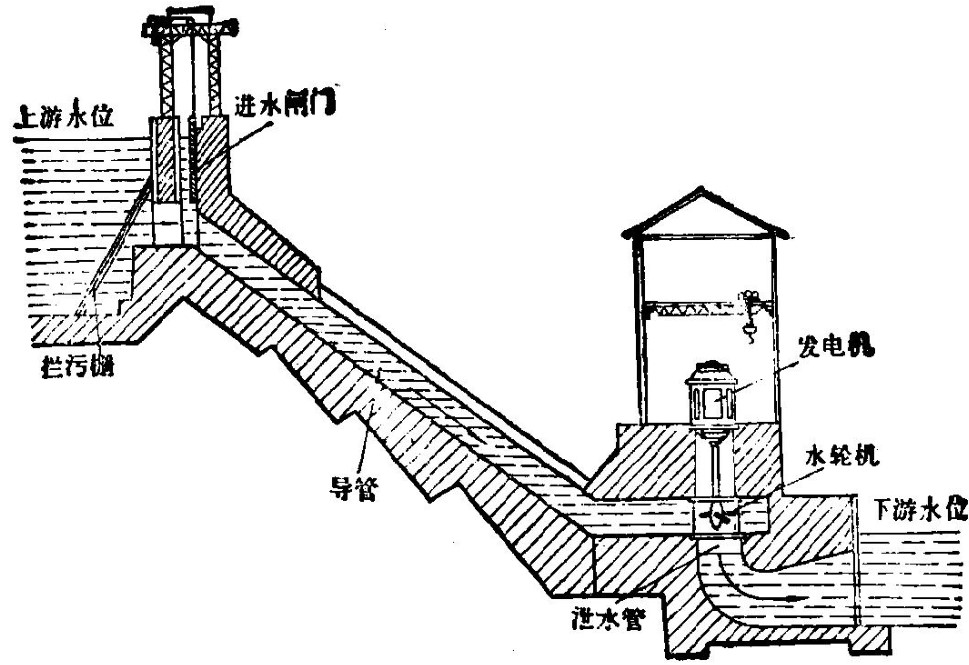
\includegraphics[width=0.8\textwidth]{../pic/czwl1-ch8-16}
    \caption{水电站剖面图}\label{fig:8-16}
\end{figure}


在一条河流上选择几个合适的地点修筑拦河坝,可以把整条河流的水能资源充分利用起来。
解放以来,在综合治理黄河的过程中就注意了水能的利用。
已经在刘家峡、盐锅峡、八盘峡、青铜峡、天桥、三门峡等地修筑了拦河大坝,建设了大型水电站,
现在正在修建龙羊峡水电站,使几千年来给两岸人民带来灾难的害河为我们的社会主义建设提供了大量的电能。
现在,我国最大的河流——长江干流的水能资源也在开发,正在兴建的葛洲坝水电站全部建成后,
安装的水轮发电机的总功率达 271.5 万千瓦。



\nonumsection{阅读材料:风能和潮汐能的利用}

任何运动的物体都有动能。流动的空气——风具有的动能叫做风能。

风能跟水能一样,都属于人类利用得最早的自然能源。
我国早在两千多年前就开始利用风来驱动帆船航行,至少在 1700 多年前已开始利用风来推动风车做工。

风能是永不枯竭的,利用起来比较筒单,不象煤炭、石油、水电那样需要开矿、钻井、筑坝,而且不会污染环境。
但是,风能不稳定,不便贮存。由于这样一些特点,风能特别适于在风力资源丰富的沿海岛屿和草原牧区,用来做允许间断的工作。
目前我国东南沿海和内蒙古草原,已经有许多小型风力发动机,用来提水灌田、碾磨谷物、加工饲料,以及带动发电机为照明、通讯供电。
图 \ref{fig:8-17} 是我国生产的 20 千瓦的风力发动机。

\begin{figure}[htbp]
    \centering
    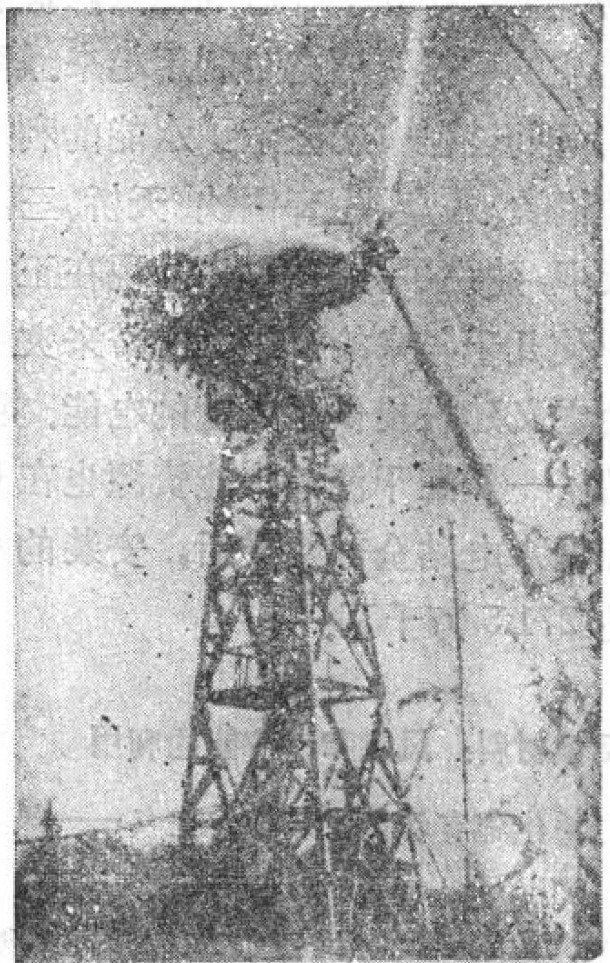
\includegraphics[width=0.5\textwidth]{../pic/czwl1-ch8-17}
    \caption{}\label{fig:8-17}
\end{figure}


潮汐能也象风能一样,是取之不尽用之不竭的,而且也不会污染环境。所谓潮汐就是海水有规律的涨落现象。
涨潮时海水上涨,大量海水奔涌而来,具有大量的动能,随着水位的逐浙升高,动能转化为势能。
退潮时海水退落,大量海水奔腾而去,势能又转化动能。
海水在这种涨落运动中具有的动能和势能就是潮汐能。

潮汐能可以用来推动水磨、水车,但是现在潮汐能利用的主要方向是发电。
利用潮汐发电跟利用河水发电类似,在海湾或河口建筑拦潮大坝,形成水库,
在坝中修建机房,安装水轮发电机,利用水位差使海水推动水轮机发电。

潮汐发电不象火力发电那样需要运输燃料,又不象河流发电那样要淹没良田、迁徙人口,还能收到海产养殖等各种效益。
但是,潮汐发电受潮水涨落影响,不均衡稳定。海水对水轮机及其他金属构件的腐蚀较大,水库泥沙淤积问题也比较严重。
这些问题都需要进一步研究,寻找更好的解决办法。所以潮汐发电现在还处于试验阶段。

我国海岸线长达 18\;000 多千米,潮汐能资源十分丰富。
现在,我国沿海省份已经修建了一些中小型潮汐电站,为进一步开发丰富的潮涉能积累经验。


